\documentclass{beamer}
\usepackage[utf8]{inputenc}
\usepackage{graphicx}

\title{Google Easy AI Framework}
\subtitle{Streamlining Data Gathering and Expert Model Creation}
\author{Franklin D.}
\date{\today}

\begin{document}

\maketitle

\begin{frame}{Introduction}
  \begin{itemize}
    \item Centralizing data from various sources.
    \item Leveraging Google Products (NotebookLM, Gemini).
    \item Creating "Expert Gems" informed by the latest sources.
  \end{itemize}
\end{frame}

\begin{frame}{Architecture Overview}
  \centering
  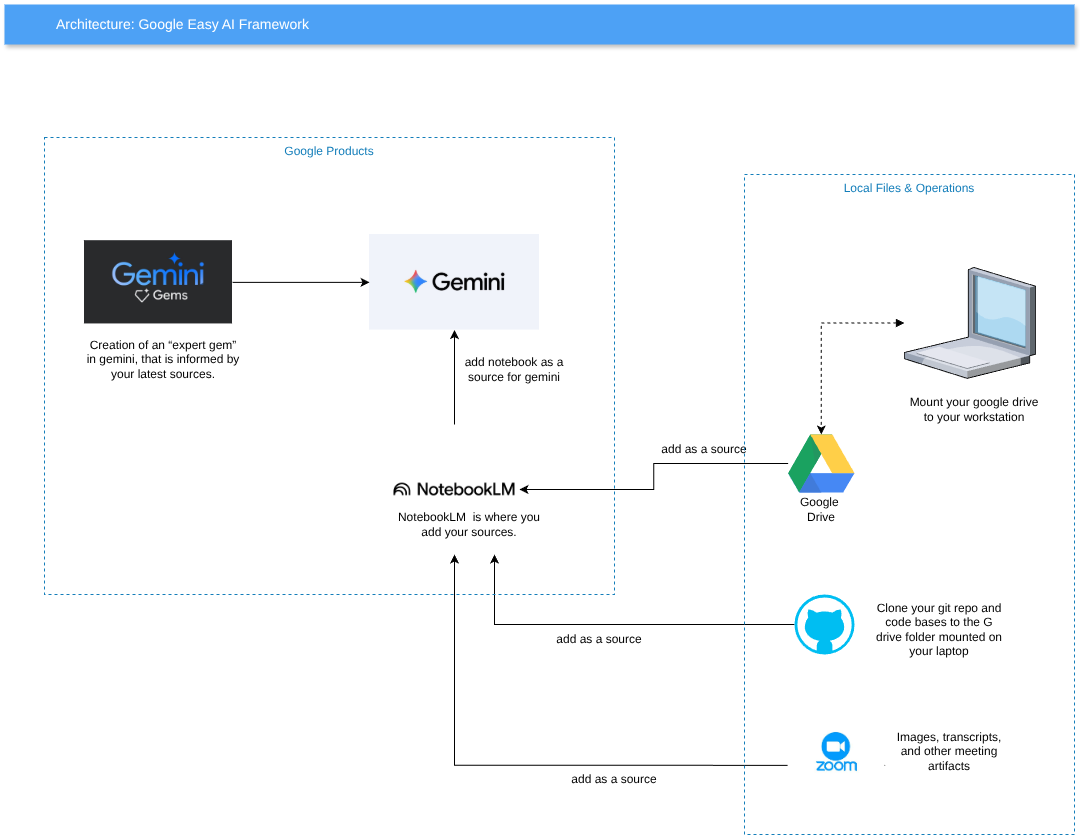
\includegraphics[width=0.8\textwidth]{../framework-google.png}
\end{frame}

\begin{frame}{Gathering the Data}
  \begin{itemize}
    \item \textbf{Zoom:} Add links to Zoom artifacts (recordings, transcripts).
    \item \textbf{Google Drive:} Mount to your workstation and add as a source.
    \item \textbf{Git Repositories:} Clone code bases (GitHub, Bitbucket, GitLab) to your local environment.
  \end{itemize}
\end{frame}

\begin{frame}{NotebookLM Integration}
  \begin{itemize}
    \item NotebookLM is the central source for your data.
    \item Add Google Drive, Zoom, and local files as sources.
    \item These sources provide the grounding for your AI interactions.
  \end{itemize}
\end{frame}

\begin{frame}{Gemini and Expert Gems}
  \begin{itemize}
    \item Gemini uses NotebookLM as a source.
    \item Creation of an "Expert Gem" in Gemini.
    \item Informed by the latest sources from your data gather.
  \end{itemize}
\end{frame}

\begin{frame}{Conclusion}
  \begin{itemize}
    \item Streamlined workflow from data collection to AI insight.
    \item Scalable architecture for incorporating diverse data sources.
  \end{itemize}
\end{frame}

\end{document}
